\documentclass[tikz,border=8pt]{standalone}
% Shared look for every TikZ diagram. Load with \input{../../tools/tikz-style.tex}
\usepackage[T1]{fontenc}
\usepackage{lmodern}
\renewcommand{\sfdefault}{lmr}  % diagrams use the same serif as the text
\usetikzlibrary{arrows.meta, positioning, shapes.geometric, calc, fit, backgrounds}
\definecolor{cblue}{HTML}{4C78A8}
\definecolor{corange}{HTML}{F58518}
\definecolor{cgreen}{HTML}{54A24B}
\definecolor{cred}{HTML}{E45756}
\definecolor{cpurple}{HTML}{B279A2}
\definecolor{cgrey}{HTML}{6B6B6B}
\tikzset{
  every picture/.style={font=\sffamily, line width=1.2pt},
  box/.style={draw=#1, fill=#1!12, rounded corners=4pt, align=center, inner sep=7pt, minimum height=1.1cm},
  box/.default=cgrey,
  arrow/.style={-{Stealth[length=3mm]}, draw=cgrey, line width=1.4pt},
  title/.style={font=\sffamily\bfseries\Large},
  note/.style={font=\sffamily\small, text=cgrey, align=center},
}
\AtBeginDocument{\hyphenpenalty=10000 \exhyphenpenalty=10000}

\begin{document}
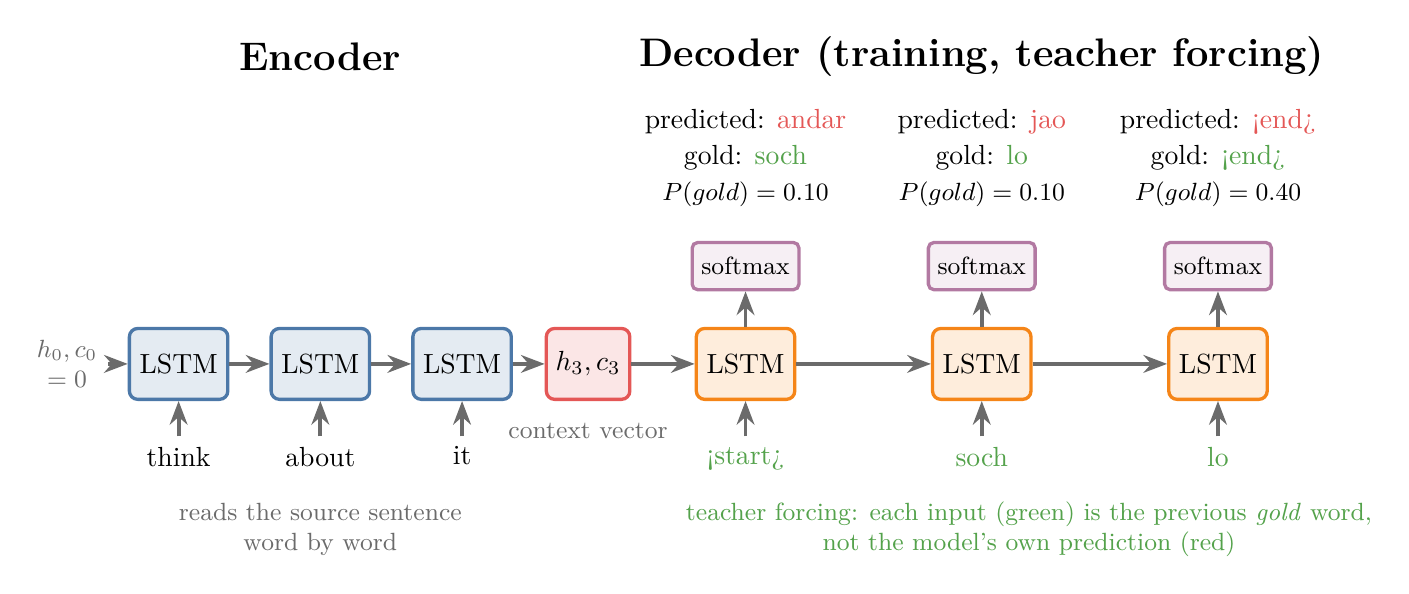
\begin{tikzpicture}[cell/.style={draw=#1, fill=#1!15, minimum width=1.25cm, minimum height=0.9cm, rounded corners=3pt, font=\sffamily},
  word/.style={font=\sffamily}, sm/.style={draw=cpurple, fill=cpurple!12, minimum width=1.25cm, minimum height=0.6cm, rounded corners=2pt, font=\sffamily\small}]
  % encoder
  \node[title] at (2.6, 3.9) {Encoder};
  \node[title] at (11.0, 3.9) {Decoder (training, teacher forcing)};
  \foreach \w [count=\i] in {think, about, it} {
    \node[cell=cblue] (e\i) at (1.8*\i - 1.0, 0) {LSTM};
    \node[word, below=0.45cm of e\i] (x\i) {\w};
    \draw[arrow] (x\i) -- (e\i);
  }
  \node[note, left=0.25cm of e1] (h0) {$h_0, c_0$\\$= 0$};
  \draw[arrow] (h0) -- (e1);
  \draw[arrow] (e1) -- (e2); \draw[arrow] (e2) -- (e3);
  \node[draw=cred, fill=cred!15, rounded corners=3pt, minimum height=0.9cm, font=\sffamily] (c) at (6.0, 0) {$h_3, c_3$};
  \node[note, below=0.15cm of c] {context vector};
  \draw[arrow] (e3) -- (c);
  % decoder
  \foreach \w/\g/\p/\pr [count=\i] in {{<start>}/soch/andar/0.10, soch/lo/jao/0.10, lo/{<end>}/{<end>}/0.40} {
    \node[cell=corange] (d\i) at (5.0 + 3.0*\i, 0) {LSTM};
    \node[word, below=0.45cm of d\i, text=cgreen] (y\i) {\w};
    \draw[arrow] (y\i) -- (d\i);
    \node[sm, above=0.45cm of d\i] (s\i) {softmax};
    \draw[arrow] (d\i) -- (s\i);
    \node[word, above=0.3cm of s\i, align=center] (p\i) {predicted: \textcolor{cred}{\p}\\[1pt]gold: \textcolor{cgreen}{\g}\\[1pt]\small $P(\text{gold}) = \pr$};
  }
  \draw[arrow] (c) -- (d1); \draw[arrow] (d1) -- (d2); \draw[arrow] (d2) -- (d3);
  \node[note, text=cgreen] at (11.6, -2.1) {teacher forcing: each input (green) is the previous \emph{gold} word,\\not the model's own prediction (red)};
  \node[note] at (2.6, -2.1) {reads the source sentence\\word by word};
\end{tikzpicture}
\end{document}
